\documentclass[11pt]{article}

\usepackage[margin=1in]{geometry}
\usepackage{setspace}
\onehalfspacing
\usepackage{graphicx}
\graphicspath{report_images/}
\usepackage{appendix}
\usepackage{listings}
\usepackage{float}
\usepackage{amsthm}
% The next three lines make the table and figure numbers also include section number
\usepackage{chngcntr}
\counterwithin{table}{section}
\counterwithin{figure}{section}
% Needed to make titling page without a page number
\usepackage{titling}

% DOCUMENT INFORMATION =================================================
\font\titleFont=cmr12 at 11pt
\title {{\titleFont ECEN 429: Introduction to Digital Systems Design Laboratory \\ North Carolina Agricultural and Technical State University \\ Department of Electrical and Computer Engineering}} % Declare Title
\author{\titleFont Reporter: Nikiyah Beulah \\ \titleFont Partner: Chris Cannon} % Declare authors
\date{\titleFont February 15, 2018}
% ======================================================================

\begin{document}

\begin{titlingpage}
\maketitle
\begin{center}
	Lab 4
\end{center}
\end{titlingpage}

\section{Introduction}
The object of this lab is to introduce students to the topic of memory and show how we might represent and handle memory in VHDL. This lab also reiterated important important concepts about components that will be utilized in this project. By the end of this lab, we will be able to implement a basic memory module in VHDL with the ability to select specific values from the memory address.

\section{Background, Design Solution, and Results}

\subsection{Problem 1 ROM Implementation}

\subsubsection{Background}
We were instructed to implement a ROM module with a 4-bit input and a 3-bit output. Because there are 4-inputs, which correspond with the available addresses in this memory. 4-bits corresponds with 2\textsuperscript{4}, or 16 possible values. Therefore, we were able to derive that there are 16 addresses in this memory module. Because the output is only 3 bits, we knew that our memory word size was 3 bits, meaning that each memory address held 3 bits of data.

\subsubsection{Design Solution}

The design we came up with for this ROM is a simple case statement what will retrieve a different value for each address. To populate our ROM for testing purposes, we decided to simply start with output "000" and iterate to "111", twice. It should be noted that the output values are trivial in this assignment. The point is to return a value stored at a given address, but the actual data stored there does not matter for this assignment. Students attempting to recreate this lab are encouraged to come up with their own values for output if they wish. The truth table for the ROM is shown in Table ~\ref{tab:romTruthTable} and the port assignments are summarized in Table ~\ref{tab:romPorts}.

\begin{table}[h]
\begin{center}
\begin{tabular}{| l | l | l | l | l |}
	\hline
	a3 & a2 & a1 & a0 & output \\ \hline
	0 & 0 & 0 & 0 & 000 \\ \hline
	0 & 0 & 0 & 1 & 001 \\ \hline
	0 & 0 & 1 & 0 & 010 \\ \hline
	0 & 0 & 1 & 1 & 011 \\ \hline
	0 & 1 & 0 & 0 & 100 \\ \hline
	0 & 1 & 0 & 1 & 101 \\ \hline
	0 & 1 & 1 & 0 & 110 \\ \hline
	0 & 1 & 1 & 1 & 111 \\ \hline
	1 & 0 & 0 & 0 & 000 \\ \hline
	1 & 0 & 0 & 1 & 001 \\ \hline
	1 & 0 & 1 & 0 & 010 \\ \hline
	1 & 0 & 1 & 1 & 011 \\ \hline
	1 & 1 & 0 & 0 & 100 \\ \hline
	1 & 1 & 0 & 1 & 101 \\ \hline
	1 & 1 & 1 & 0 & 110 \\ \hline
	1 & 1 & 1 & 1 & 111 \\ \hline
\end{tabular}
\caption{\label{tab:romTruthTable}Truth table for our ROM implementation.}
\end{center}
\end{table}

\begin{table}[h]
\begin{center}
\begin{tabular}{| l | l | l |}
	\hline
	Bit & Label & Port \\ \hline
	a3 & Switch 3 & W17 \\ \hline
	a2 & Switch 2 & W16 \\ \hline
	a1 & Switch 1 & V16 \\ \hline
	a0 & Switch 0 & V17 \\ \hline
	o2 & LED 2 & U19 \\ \hline
	o1 & LED 1 & E19 \\ \hline
	o0 & LED 0 & U16 \\ \hline
\end{tabular}
\caption{\label{tab:romPorts}Port assignments for ROM implementation.}
\end{center}
\end{table}

\subsubsection{Results}

\subsection{Problem 2 ROM Multiplexer}

\subsubsection{Background}

\subsubsection{Design Solution}

\subsubsection{Results}

\section{Conclusion}

\pagebreak

\textbf{Appendices}

\begin{appendices}

\section{Problem 1 VHDL Code}

\begin{lstlisting}[language=VHDL]
library IEEE;
use IEEE.STD_LOGIC_1164.ALL;

entity rom is
    Port ( a : in STD_LOGIC_VECTOR(3 downto 0);
           o : out STD_LOGIC_VECTOR(2 downto 0));
end entity rom;

architecture rom_arch of rom is
    
begin
process(a)
    begin
        case a is
            when "0000" => o <= "000";
            when "0001" => o <= "001";
            when "0010" => o <= "010";
            when "0011" => o <= "011";
            when "0100" => o <= "100";
            when "0101" => o <= "101";
            when "0110" => o <= "110";
            when "0111" => o <= "111";
            when "1000" => o <= "000";
            when "1001" => o <= "001";
            when "1010" => o <= "010";
            when "1011" => o <= "011";
            when "1100" => o <= "100";
            when "1101" => o <= "101";
            when "1110" => o <= "110";
            when "1111" => o <= "111";
        end case;
    end process;
end rom_arch;
\end{lstlisting}

\section{Problem 1 Constraints File}
\begin{figure}[H]
\begin{center}
	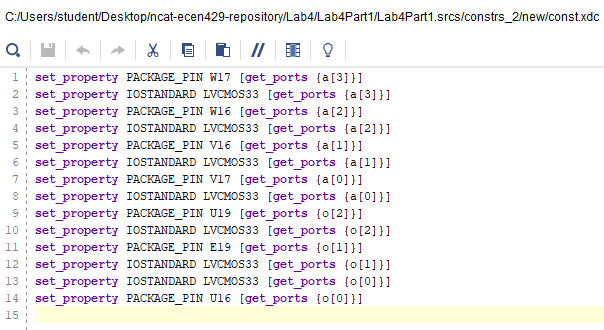
\includegraphics[width=0.5\textwidth]{../report-images/Part1Const.png}
	\caption{\label{fig:Part1ConstFile}Constraints file for Problem 1.}
\end{center}
\end{figure}

\section{Problem 2 VHDL Code}
\begin{lstlisting}[language=VHDL]
library IEEE;
use IEEE.STD_LOGIC_1164.ALL;

entity rom is
    Port ( a : in STD_LOGIC_VECTOR(3 downto 0);
           o : out STD_LOGIC_VECTOR(2 downto 0));
end entity rom;

architecture rom_arch of rom is
    
begin
process(a)
    begin
        case a is
            when "0000" => o <= "000";
            when "0001" => o <= "001";
            when "0010" => o <= "010";
            when "0011" => o <= "011";
            when "0100" => o <= "100";
            when "0101" => o <= "101";
            when "0110" => o <= "110";
            when "0111" => o <= "111";
            when "1000" => o <= "000";
            when "1001" => o <= "001";
            when "1010" => o <= "010";
            when "1011" => o <= "011";
            when "1100" => o <= "100";
            when "1101" => o <= "101";
            when "1110" => o <= "110";
            when "1111" => o <= "111";
        end case;
    end process;
end rom_arch;

library IEEE;
use IEEE.STD_LOGIC_1164.ALL;

entity rom_mux is
    Port ( x : in STD_LOGIC_VECTOR(3 downto 0);
           sel : in STD_LOGIC_VECTOR(1 downto 0);
           z : out STD_LOGIC_VECTOR(6 downto 0));
end rom_mux;

architecture Behavioral of rom_mux is
component rom is port(a : in STD_LOGIC_VECTOR(3 downto 0); 
	o : out STD_LOGIC_VECTOR(2 downto 0));
end component rom;

signal val : STD_LOGIC_VECTOR(2 downto 0);

begin
    rom_com : rom port map(x, val);
    process(sel)
        begin
            case sel is
                when "00" => 
                    if(val(0) = '1') then z <= "1001111";
                    else z <= "0000001";
                    end if;
                when "01" =>
                    if(val(1) = '1') then z <= "1001111";
                    else z <= "0000001";
                    end if;
                when "10" => 
                    if(val(2) = '1') then z <= "1001111";
                    else z <= "0000001";
                    end if;
                when others => z <= "0000000";
            end case;
    end process;
end Behavioral;
\end{lstlisting}

\section{Problem 2 Constraints File}
\begin{figure}[H]
\begin{center}
	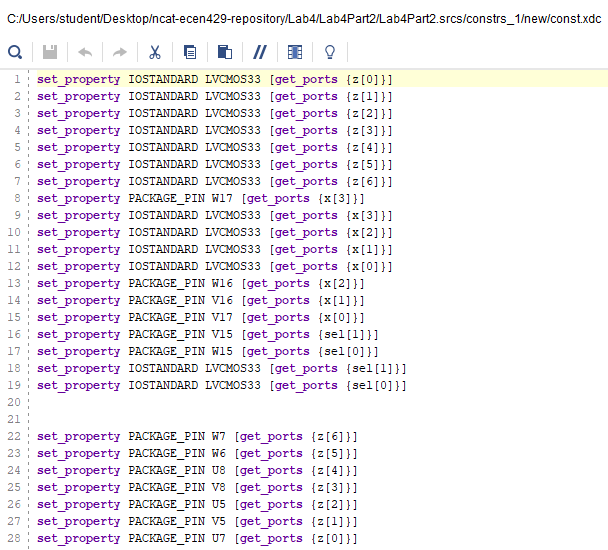
\includegraphics[width=0.5\textwidth]{../report-images/Part2Const.png}
	\caption{\label{fig:Part2ConstFile}Constraints file for Problem 2.}
\end{center}
\end{figure}

\end{appendices}
\end{document}
